
% Example pseudo-code from the original thesis template:
% \begin{algorithm}
%     \begin{algorithmic}
%     \Function{ExecuteWithHighProbability}{$A$}
%         \State $r \gets$ a random number between $0$ and $1$
%         \State $\varepsilon \gets 0.0000000000000000000000000000000000000042$
%         \If{$r\geq\varepsilon$}
%             \State execute $A$ \Comment{We discard the return value}
%         \Else
%             \State print: \texttt{Not today, sorry.}
%         \EndIf
%     \EndFunction
%     \end{algorithmic}
%     \caption{Algorithm that executes an action with high probability. Do not care about formal semantics in the pseudocode --- semicolons, types, correct function call parameters and similar nonsense from `realistic' languages can be safely omitted. Instead make sure that the intuition behind (and perhaps some hints about its correctness or various corner cases) can be seen as easily as possible.}
%     \label{alg:w}
% \end{algorithm}



\chapter{Background}
\label{chap:background}

% \xxx{In this chapter we discuss the related work in the field of subword tokenization and multilingual pretrained models. We start with a brief overview of the subword tokenization methods and then discuss the multilingual pretrained models. We also discuss the work that has been done in the field of multilingual subword tokenization.}

% In order to organize Chapter Two, you will first start with an introduction about the general problem and your topic. Then you will provide an advance organizer, which indicates what will be covered in the literature review.

In this thesis we investigate the effect of subword tokenization on the performance of multilingual pretrained models. To that end we first introduce the reader to the recent field of pretrained language models and cross-lingual models. We explain the concept of subword tokenization and the most common subword tokenization methods. Lastly, we show what problems arise when using pretrained models in multilingual settings and what methods have been proposed to mitigate these problems.


\section{Language representation models}

In recent years we have seen a dramatic rise in the use of neural language models. The premise of these models is the ability to learn effectively from large amounts of unlabeled data. 

\xxx{TODO}

Language modeling is a task where we predict the next word given the previous words. \cite{manning_foundations_1999} More formally, given a sequence of words $w_1, w_2, \dots, w_{m-1}$, the language model computes the probability of the next word $w_{m}$:

\begin{equation}
    P(w_{m} | w_1, w_2, \dots, w_{m-1})
\end{equation}

One method to compute this probability is to use n-gram language models. These models simplify the problem by making a Markov assumption --- the probability of the next word is conditioned only on the previous $n-1$ words:

\begin{equation}
    P(w_{m} | w_1, w_2, \dots, w_{m-1}) \approx P(w_{m} | w_{m-n+1}, w_{m-n+2}, \dots, w_{m-1})
\end{equation}

\xxx{TODO}

terms I use later that need explaination:
- embedding layer of mBERT, embedding matrix
- model size
- masked language models

\section{Multilingual pretrained models}

\xxx{TODO}

\subsection{Assessing the ability of multilingual models}

- word level tasks
- sentence level tasks
- inlanguage vs crosslingual

\section{Subword tokenization}

Subword tokenization methods split up words into subword units, which are then used as the input tokens for the neural models. This is done to mitigate the out-of-vocabulary (OOV) problem and to reduce the computational complexity of the softmax cross-entropy loss over a very large output vocabulary. The most common subword tokenization methods are Byte Pair Encoding (BPE), Unigram LM and Wordpiece.

\xxx{TODO: define vocabulary - set of all tokens, vocabulary size}

\subsection{Byte Pair Encoding (BPE)}

The Byte Pair Encoding (BPE) algorithm was introduced by \citet{Sennrich2015}. They have adapted a compression algorithm \todo{cite Gage 1994} to learn a subword vocabulary from a corpus. This method was shown to improve the performance of neural machine translation (NMT) models. BPE was subsequently used for some of the well known pretrained models such as GPT-2 \citep{Radford2019}.

The principle of BPE is to iteratively merge the most frequent byte pairs in the corpus until the vocabulary size reaches the target size. The algorithm starts with a vocabulary of unique characters used in the input corpus. Using this vocabulary, we then compute the frequency of every character pair and merge the most frequent pair to create a new subword unit. We recompute the frequency of the subword unit pairs and repeat the process until the target vocabulary size is reached.

\xxx{add info about inference}

\begin{algorithm}
    \begin{algorithmic}
        \Function{BPE}{$C$}
        \State $V \gets$ unique characters in $C$
        \While{$|V| < V_{target}$}
        \State $p \gets$ most frequent pair in $V$
        % \State $V \gets V \setminus p$
        \State $V \gets V \cup \{p\}$
        \EndWhile
        \State \Return $V$
        \EndFunction
    \end{algorithmic}
    \caption{The Byte Pair Encoding algorithm.}
    \label{alg:bpe}
\end{algorithm}

% \subsection{Byte-level BPE}


\subsection{Wordpiece}

First introduced in \cite{SchusterandNakajima2012)} the Wordpiece algorithm is a similar technique to BPE. It is used in the well known pretrained models such as BERT \citep{devlin_bert_2019}. The training is based on greedy merging of the subword units. Unlike BPE, Wordpiece does not use the frequency of the subword units to merge them. Instead, it merges the pair that maximizes the likelihood of an n-gram language model trained on the corpus.

Contrary to BPE and Unigram LM, there is no official, public implementation of the original Wordpiece algorithm. There are several implementations of the algorithm available but these diverge from the original algorithm. For example, the implementation in the HuggingFace library \citep{wolf_transformers_2020} does not use the n-gram language model to merge the subword units. Instead, the training follows the BPE procedure and only adds prefixes to the subword units to mimic the output format of the BERT Wordpiece implementation. \xxx{add a link into the source code?}

The implementation in the Tensorflow library follows a top-down approach to create the subword vocabulary. It starts with a vocabulary of words and then iteratively splits the words into subword units to reach a target vocabulary size.

\xxx{add inference}

\subsection{Unigram LM}

The Unigram LM tokenizer, sometimes referred to as the SentencePiece tokenizer \citep{kudo_sentencepiece_2018}, was introduced by \citet{kudo_subword_2018}. The motivation for this method was to create a probabilistic model for subword tokenization. With this model, it is then possible to sample different segmentations of the input text. Training on these varied segmentations empirically improves the performance of the NMT models. In large language models such as XLM-R, the Unigram tokenizer is used deterministically, always choosing the most probable segmentation.

Given an input sentence $X$, the Unigram LM algorithm finds the most probable segmentation $x^\star$ for the input sentence X:

\begin{equation}
    x^\star = {\arg\max}_{x \in \mathcal{S}(X)} P(x)
\end{equation}


Where $\mathcal{S}(X)$ is the set of all possible segmentations of the input sentence $X$ given a subword vocabulary $\mathcal{V}$. The probability $P(x)$ of a segmentation $x$ is computed as a product of subword occurrence probabilities $p(x_i)$:

\begin{equation}
    P(x) = \prod_{i=1}^{|x|} p(x_i)
\end{equation}

Here, the subword occurence probabilities cannot be computed using occurence statistics in the corpus. With a given vocabulary, there is usually many possibilites on how to segment the input sentence from character level granularity to word level. Instead, the Unigram LM uses the Expectation-Maximization (EM) algorithm to estimate the subword occurrence probabilities $p(x_i)$. The EM algorithm maximizes the marginal likelihood $\mathcal{L}$ with respect to the latent subword probabilities $p(x_i)$:

\begin{equation}
    \mathcal{L} = \sum_{s=1}^{|D|} \log (P(X^{(s)})) = \sum_{s=1}^{|D|} \log( \sum_{x \in \mathcal{S}(X^{(s)})} P(x) )
\end{equation}

By maximizing the marginal likelihood, the Unigram LM considers all possible segmentations of the input sentences when estimating the subword occurrence probabilities $p(x_i)$. After optimization of $p(x)$, it is then possible to compute the most probable segmentation $x^\star$ for a given input sentence $X$ using the Viterbi algorithm.

The training of the Unigram LM works in a top-down fashion. It starts with a large seed vocabulary of the most frequent character n-grams. These character n-grams are then iteratively pruned down to the target vocabulary size in the following way:

\begin{enumerate}
    \item With a given vocabulary $\mathcal{V}$, estimate the subword occurrence probabilities $p(x_i)$ using the EM algorithm.
    \item Segment the training corpus, sample the best segmentation for every sentence.
    \item For each subword $x_i$ in the vocabulary, compute the loss. The loss is defined as the decrease in the unigram language model likelihood if the subword is removed from the vocabulary.
    \item Keep the top 80\% of the subwords with the lowest loss.
    \item Repeat this process with the new vocabulary $\mathcal{V}$ until the target vocabulary size is reached.
\end{enumerate}

\xxx{-> bostrom has really nice pseudocode}

% For a given vocabulary $\mathcal{V}$,

% The pruning is done using a unigram language model. With a subword vocabulary and corresponding subword occurence probabilities $p(x_i)$, the unigram language model computes the probability of a sentence $X$ as follows:

% The Unigram LM algorithm uses, as the name suggests, a unigram language model to learn the subword vocabulary. 


% With the default hyperparameter settings, the algorithm starts with an initial vocabulary of $1 000 000$ \todo{fix num} most frequent character ngrams found within the word boundaries. These character n-grams are then iteratively pruned down to the target vocabulary size. T

% The overview of the algorithm is as follows:

% 1. Create a large seed vocabulary

% 2. Repeat until the target vocabulary size is reached:


% (a). Optimize the subword occurence probabilities $p(x_i)$ using the EM algorithm (default value is 2 EM subiterations). The EM algorithm maximizes the marginal likelihood $\mathcal{L}$ with $p(x_i)$ as the latent variables:

% Expectation step: Compute the marginal probability of each subword $x_i$ using the current probabilities $p(x_i)$.

% Maximization step: Compute the new probabilities $p(x_i)$ using the expected number of occurrences $E(x_i)$.

% (b). Merge the n-gram with the highest probability

% Under the assumptions of the unigram language model, the probability of a sequence $x = ( x_1, \dots, x_n )$ is given by the product of the probabilities of the individual tokens $x_i$:

% \begin{equation}
%     P(x) = \prod_{i=1}^{n} P(x_i)
% \end{equation}

% The initial probability of the character n-grams is given by their frequency in the corpus over the sum of all frequencies:

% \begin{equation}
%     P(x_i) = \frac{f(x_i)}{\sum_{j=1}^{N} f(x_j)}
% \end{equation}

\subsection{Alternative tokenization approaches (low priority)}

\subsubsection{Character-level models}
\subsubsection{Morphology based models}

\section{Subword regularization (low priority)}

\begin{enumerate}
    \item bpe dropout
    \item unigram lm
\end{enumerate}


% \chapter{Related work}
% \label{chap:related_work}

\section{Tokenization with many languages}

Despite the recent advances in language modeling, the tokenization methods used in the multilingual language models remain mostly unchanged. The first models trained on multiple languages, such as mBERT \cite{devlin_bert_2019} and XLM \cite{lample_cross-lingual_2019} use the same tokenization methods as their monolingual versions - namely the Wordpiece and BPE algorithms. Later language models such as XLM-R \cite{conneau_unsupervised_2020}, mBART \cite{liu_multilingual_2020} or mT5 \cite{xue_mt5_2021} use the Unigram LM algorithm to learn the subword vocabulary. The most recent multilingual generative models, such as the 176B parameter BLOOM model \cite{scao_bloom_2022} or the XGLM \cite{lin_few-shot_2022} use the Byte-level BPE and Unigram LM algorithms respectively.


% - section about how language models are still using the tokenization techniques such as BPE and Unigram LM that were developed for monolingual models.
% - example models: mBERT uses Wordpiece, XLM uses BPE, XLM-R uses Unigram LM. More curHow can we evaluate and improve them?  (va, vo)
% - mBART uses Unigram LM, T5 and mT5 uses Unigram LM. Even more recently, the 176B parameter BLOOM model uses Byte-level BPE and the multilingual generative model XGLM uses Unigram LM. Most of these models use the SentencePiece implementation and run the tokenization algorithm on the concatenation of all languages in the training data.


The methods these models use to tokenize the input text are the same as the ones used in the monolingual models. The main difference is that the tokenization training algorithm is run on all of pretraining data. This means that the tokenizer is trained on all languages at once. 

As we have pointed out previously, the pretraining data is not evenly distributed across languages. High resource languages such as English or Indonesian may have hundreds times the amount of training data than low resource languages such as Swahili or Amharic. To account for the discrepancy in the number of training examples per language, the training data is usually subsampled with a bias towards low-resource languages. This subsampling is performed both for the model pretraining and the tokenizer training \cite{devlin_bert_2019,lample_cross-lingual_2019}. \xxx{cite maybe the mBERT github page rather than bert paper. But I don't know how to cite it pls help}

We describe the subsampling method in detail in Section \ref{sec:data_scope}. In a nutshell, the subsampling is done by adjusting the probability of sampling a line $p(l)$ from a language $l$. The probabilities are exponentiated with a factor $\alpha$ and renormalized to sum to 1. With $\alpha=0.0$, the subsampling is uniform across languages. With $\alpha=1.0$, the smoothing has no effect. The usual values chosen for this factor $\alpha$ are 0.7 \cite{devlin_bert_2019}. 0.5 \cite{lample_cross-lingual_2019} and 0.3 \cite{conneau_unsupervised_2020}.

\subsection{Bias towards high-resource languages}

As \citet{rust_how_2021} have shown, the bias towards high-resource however still persists. \citet{rust_how_2021} compare the performance of the multilingual model mBERT and language specific variants of BERT. By finetuning and evaluating on five different tasks across nine typologically different langugaes, they show that there is a performance gap between the multilingual and monolingual models. By further examination they determine that the performance gap may be explained by 1) pretraining data size and 2) the choice of tokenizer and its suitability for the tested language. 

They show that the performance of mBERT can be improved for a specific language by switching to a monolingual vocabulary and retraining only the embedding layer of mBERT. The model with a dedicated vocabulary outperforms the vanilla mBERT on a variety of tasks, which indicates that the multilignual vocabulary of mBERT is not optimal. 

But what changes when we switch to a monolingual vocabulary and why does it improve the multilingual model to the point it approaches the performance of the dedicated monolingual model? \citet{rust_how_2021} propose to look at how often the tokenizer segments words. They show that for some languages, the multilingual tokenizer splits words into subwords drastically more often than the monolingual tokenizer. By changing the tokenizer, we improve the tokenization of the input text and thus the model performance.

For measuring this, \citet{rust_how_2021} use a metric called \textit{fertility} \cite{acs_exploring_2019}. It is defined as the average number of subwords per word. They show that the fertility of the multilingual tokenizer is higher than the fertility of the monolingual tokenizer, especially for low-resource languages that are underrepresented in the training data. By measuring the correlation between the improvement in performance of the modified models and improvement in fertility, they show that there is a statistically significant relationship between the two.
% They also show that the downstream task performance is negatively affected by how often the tokenizer splits single words into several subwords. For this they use a metric called \textit{fertility} \cite{acs_exploring_2019}. It is defined as the average number of subwords per word.

% By comparing the fertility metric \citet{rust_how_2021} has shown that oversegmentation oversegmentation of low-resource languages leads to longer sequence lengths and more frequent splitting of words. Thus the multilingual model must learn to compose the subwords back into semantic units and also learn to attend to correct subwords over longer distances \cite{chung_improving_2020}. Moreover, mismatched segmentation granularity might lead to incompatible representations for subwords across languages. \citet{maronikolakis_wine_2021} have shown that tokenization compatibility can have a significant impact on multilingual performance.

\section{Mitigating the language bias}

As we have described, \citet{rust_how_2021} have firmly established that there is indeed a disparity between the performance of the multilingual model mBERT and similar monolingual models. They have shown that the disparity is in part caused by the tokenization method used in the multilingual model.

Other works have addressed this issue by proposing novel tokenization methods, that aim to improve the vocabulary of the multilingual model and increase its size to accomodate for all represented languages. The works of \citet{chung_improving_2020,zheng_allocating_2021,liang_xlm-v_2023} all introduce new multilingual models that use an expanded vocabulary and a novel tokenization method for mitigating the language bias. Moreover, the authors all show that the standard recipe of training a tokenizer on a concatenation of all languages in the training data is not optimal and that the performance of the model can be improved by using their method, especially for the low-resource languages.

In the following subsections, we will describe these three methods. First, we describe the method of \citet{chung_improving_2020}, which replaces the standard method with a procedure of clustering similar language corpora together and training separate cluster-tokenizers before merging these tokenizers together. Then we describe the method introduced by \citet{zheng_allocating_2021} which infers the optimal per-language vocabulary size and then trains separate, monolingual tokenizers for each language that are then merged. Lastly, we describe the method of \citet{liang_xlm-v_2023}, which combines the previous two methods and trains even larger vocabularies than the previous two methods.

% They have also shown that the disparity can be mitigated by switching to a monolingual vocabulary. However, this is not a viable solution for multilingual models, as it would require a separate vocabulary for each language.

% There have been several attempts to mitigate the language bias in multilingual language models. We will now describe the most prominent ones.

\xxx{add simple explanation of the methods}

\subsection{Language-Clustered Vocabularies}

In their paper \Citetitle{chung_improving_2020} \cite{chung_improving_2020}, \citeauthor{chung_improving_2020} propose a method to effectively increase the vocabulary size while mitigating the the language bias by using language-clustered vocabularies. They construct an improved vocabulary by merging together several smaller vocabularies that were trained on subsets of the whole, multilingual training corpus. These smaller vocabularies are constructed by clustering the monolingual corpora based on their similarity and then training a separate vocabulary for each cluster. The authors show that the language-clustered vocabularies lead to improved performance on low-resource languages.


\begin{figure}[ht]
    \centering
    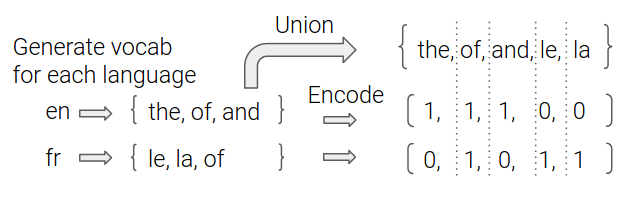
\includegraphics[width=0.5\textwidth]{img/temp/chung_language_vectors.png}
    \caption{Binary vector representations used for language clustering. Figure taken from \cite{chung_improving_2020}.}
    \label{fig:chung_vectors}
\end{figure}

Their method works by clustering the languages and then merging the cluster-level vocabularies. To cluster the languages using the k-means algorithm, it is necessary to define an euclidean vector space with each language having a representative vector (\autoref{fig:chung_vectors}). To this end, the authors first train equally sized vocabularies $V^l$ for each language separately using the Unigram LM method. Then they create a merged vocabulary $V^L$ by taking the union of the vocabularies $V^l$. Then, to produce a language vector $\vec{v}^l$ for each language $l$, the presence of each subword $V^L_i$ is checked in the language-specific $V^l$ and the value is set to 1 if the subword is present and 0 otherwise.

\begin{equation}
    \vec{v}^l_i = \begin{cases}
        1 & \text{if } V^L_i \in V^l \\
        0 & \text{otherwise}
    \end{cases}
\end{equation}

With the languages represented as vectors, the k-means algorithm can be used to cluster them. The authors use the cosine distance as the distance metric 
% (or equivalently: they normalize the language vectors to have a length 1 before clustering).
With 104 languages in total, the number of clusters is set to 8. The choice of $k$ is determined empirically by running a set of preliminary experiments and comparing the results on a multilingual question-answering benchmark. The resulting clusters are shown in \autoref{fig:chung_clusters}.

After the languages are clustered, the cluster-specific vocabularies are trained using the Unigram LM algorithm on the union of the corpora of the languages in the cluster. The size of each cluster-specific vocabulary is proportional to the size of the union of the individual (monolingual) vocabularies in the cluster. This means that more languages in a cluster lead to larger vocabulary size assigned but also if the languages share tokens, this overlap decreases the vocabulary size. The final vocabulary is then constructed by simply taking the union over the cluster vocabularies.

\begin{figure}[ht]
    \centering
    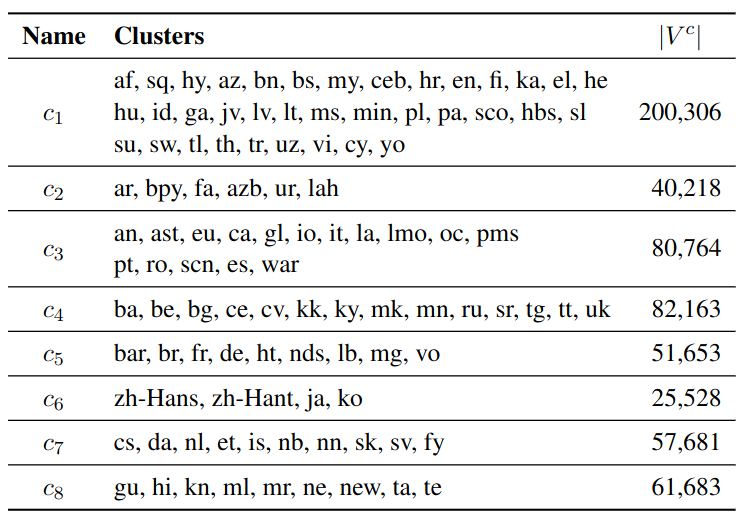
\includegraphics[width=0.8\textwidth]{img/temp/chung_clusters.png}
    \caption{Clusters of languages used in \cite{chung_improving_2020}. The clusters are numbered from 0 to 7. Figure taken from \cite{chung_improving_2020}.}
    \label{fig:chung_clusters}
\end{figure}

The final vocabulary is then compared to the standard recipe of training a Unigram LM vocabulary on a joint corpus\footnote{The authors do not define what they mean by following the "standard recipe". Based on the related work the authors replicate closely (mBERT and XLM-R) and compare themselves to, we assume that the standard recipe is training a Unigram LM tokenizer on the pretraining data after the exponential subsampling described in \ref{sec:data_scope}. The authors do mention using the sampling factor $\alpha=0.7$ for the pretraining data in the Appendix.}. Because the proposed clustering method does not have a way of controlling the size of the final vocabulary as taking the union inadvertently leads to some tokens being merged, the authors compare the vocabularies by first following the clustering method and arriving at a 488k subword vocabulary. Then the standard method is followed to train a vocabulary of the same size.

The authors evaluate the vocabularies intrinsically - by examining the average number of tokens per sentence, out-of-vocabulary rate and vocabulary overlap using the Wasserstein-1 distance.
By computing the average number of tokens per sentence for the whole corpus and for each language separately, the authors show that their method leads to a smaller average number of tokens per sentence for the whole corpus and further show that the improvements are more prominent for the low-resource languages. The authors also show that the out-of-vocabulary rate is lower for the language-clustered vocabulary, again the largest reduction in the OOV rate are in the low-resource and rare-script languages. Finally, the authors show that the language-clustered vocabulary leads to a smaller Wasserstein-1 distance between the similar languages and at the same time larger distance between the linguistically different languages.

The clustered vocabulary is then used to train a smaller and bigger multilingual masked language model and evaluated on three distinct, multilingual tasks (question answering, natural language inference and named entity recognition). The baselines selected are the original mBERT model, XLM-R model and a smaller reproduction of XLM-R with an increased vocabulary size to match the parameter size of the introduced model. The authors show improvements for the smaller model on all three tasks over their baseline reproduction. Then they show the improvements in QA and NER tasks for the bigger model over the XLM-R and mBERT baselines. 

% The authors propose a new multilingual tokenization method. The vocabulary is constructed by clustering languages, applying SentencePiece to each cluster and merging the vocabularies together.
% The clustering is done by comparing similarity between monolingual vocabularies (NOT taking frequency of tokens into account - that is done in Liang et al 2023). Target vocabulary size for each cluster is proportional to the size of the union of the individual (monolingual) vocabularies in the cluster. The final vocabulary is simply union over the cluster vocabs (how do they ensure the target size for the whole vocab?)
% Intrinsic evaluation of the alternative vocabularies is done by computing the empirical distributions of the languages using Wasserstein-1 distance. The metric is used to compare the tokenizers and to prove that in the new approach, there is a smaller distance in the similar languages and at the same time bigger distance in the linguistically different languages. They also show that the Chinese and Arabic scripts is now in a larger share of the vocabulary.
% To analyze the “vocabulary allocation” they use a reformulation of description length for tokenizers = description length is equivalent to the the vocabulary size, and the number of integers of the encoded or tokenized input data. When comparing two tokenizers with the same vocabulary size, this is equivalent to comparing the average number of tokens per sentence. Caveat: there might be tradeoff with the out of vocabulary rate. They propose DL as a proxy metric to compare vocabularies.
% this work, we introduce a novel procedure for multilingual vocabulary generation that combines the separately trained vocabularies of several automatically derived language clusters, thus balancing the trade-off between cross-lingual subword sharing and language-specific vocabularies. Our experiments show improvements across languages on key multilingual benchmark tasks TYDI QA (+2.9 F1), XNLI (+2.1\%), and WikiAnn NER (+2.8 F1) and factor of 8 reduction in out-of-vocabulary rate, all without increasing the size of the model or data.
% Notes
% Because these algorithms look at overall subword frequencies in the combined multilingual corpus, they may learn suboptimal decompositions for low-resource languages that happen to have character combinations that resemble subwords of high-resources languages.
% subwords in common scripts like Latin and Cyrillic have a higher chance of selection since their counts are combined across a large number of languages (Wu and Dredze, 2019)
% subword sharing is not the principal reason for the effectiveness of multilingual models K et al. (2020)
% Ideas:

% - This still does not seem to solve the problem with cross-lingual sharing of wrong tokens such as “a” (conj in cs vs prep in eng)
% - Can we do the clustering better so that the languages are clustered according to the  downstream performance rather than hand-picked similarity metric between langs?





\subsection{Determining vocabulary capacity for each language}

In the paper \Citetitle{zheng_allocating_2021}, \citeauthor{zheng_allocating_2021} propose a method for determining the optimal vocabulary capacity for each language in a multilingual model. Then they propose a method for constructing a multilingual vocabulary by combining monolingual vocabularies so that the optimal capacity is achieved for each language. In the second part of the paper, the authors propose a method for accelerating the training of the model with the increased vocabulary size, which is out of the scope of this thesis.

% % - they observe that multilignual models do have a larger vocabulary than monolingual models (30k to 60k vs 250k). Still it is 2.5k per language on average in xlm-r
% - they consider each language separately and calculate the optimal vocabulary size for each language
% - using subword segmentation algorithms like BPE or unigram language model → they select subword tokens shared across languages with the same script and have lower chance to select language-specific subword units


To determine the optimal vocabulary capacity for each language, the authors propose a metric called \textit{average log probability} (ALP). 

$$
ALP(\mathcal{D}_i, V) = \frac{1}{|\mathcal{D}_i|} \sum_{j=1}^{|\mathcal{D}_i|} \sum_{k=1}^{|s_j|} \log(p_{uni}(s^k_{j}))
$$

where $\mathcal{D}_i$ is the monolingual corpus of language $i$, $V$ is the vocabulary and $p_{uni}(s^k_{j})$ is the unigram probability of the $k$-th token in the $j$-th sentence. The authors show that the average log probability positively correlates with the downstream task performance on a series of experiments with four distinct languages. They show this correlation by training a series of tokenizers with an increasing vocabulary size. Then they measure the ALP on these tokenizers, pretrain monolingual models for every vocabulary size and every language and evaluate them on two word-level classification tasks. For illustration we show the correlation between ALP and F1 score for the NER task in Figure \ref{fig:alp_vs_NER}. 

% show figure 2 and 3 
% \begin{figure}[h]
%     \centering
%     \begin{minipage}{0.45\textwidth}
%         \centering
%         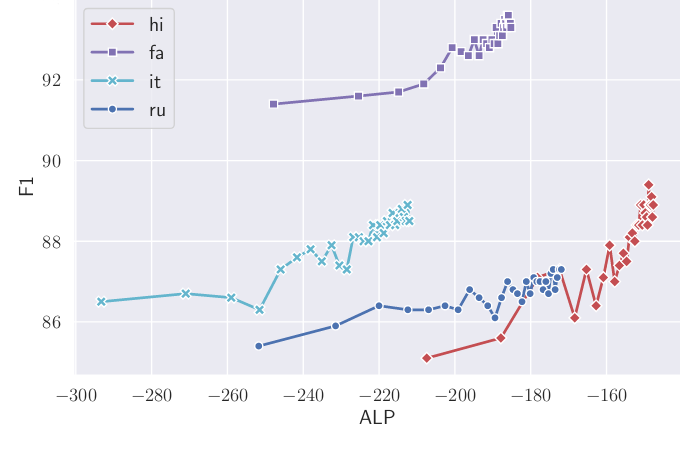
\includegraphics[width=\textwidth]{img/temp/alp_vs_NER.png}
%         \caption{F1 score on NER task with different vocabularies versus their ALP on the monolingual corpus. Figure taken from \cite{zheng_allocating_2021}}
%         \label{fig:image1}
%     \end{minipage}\hfill
%     \begin{minipage}{0.45\textwidth}
%         \centering
%         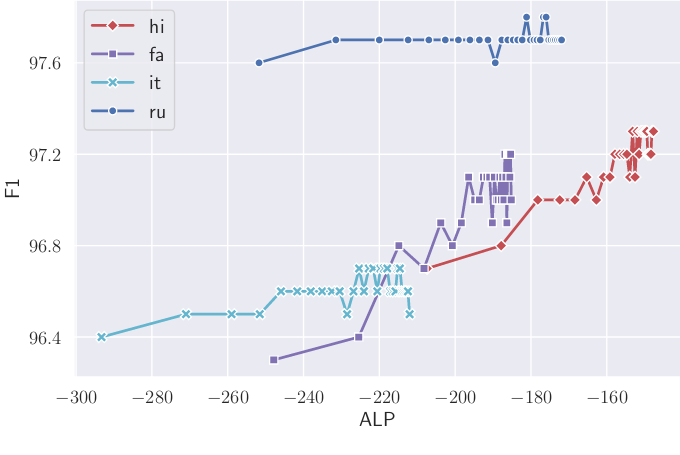
\includegraphics[width=\textwidth]{img/temp/alp_vs_POS.png}
%         % \caption{F1 score on POS task with different vocabularies versus their ALP on the monolingual corpus. Figure taken from \cite{zheng_allocating_2021}}
%         \label{fig:image2}
%     \end{minipage}
% \end{figure}

\begin{figure}[h]
    \centering
    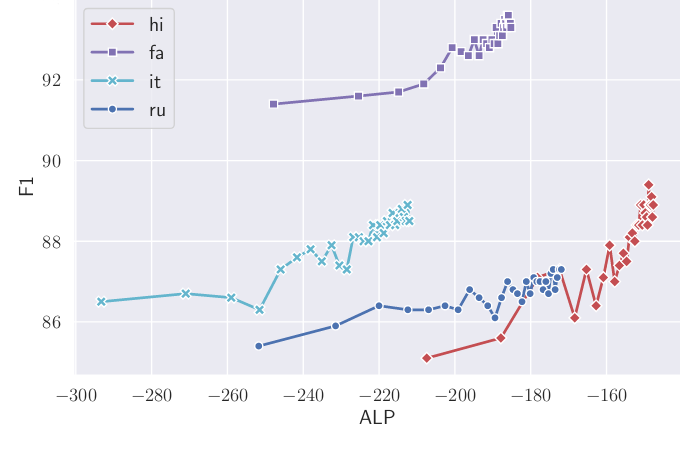
\includegraphics[width=0.65\textwidth]{img/temp/alp_vs_NER.png}
    \caption{F1 score on NER task with different vocabularies versus their ALP on the monolingual corpus. Figure taken from \cite{zheng_allocating_2021}}
    \label{fig:alp_vs_NER}
\end{figure}

Although the authors report that the vocabulary size itself is also a good predictor of downstream task performance, the authors argue that ALP correlates better with the downstream task performance and is therefore a better metric for determining the optimal vocabulary capacity.

%     - ALP correlates positively with downstream task performance
% - correlates better than only comparing vocabulary size
% - here they must compare pearson correlation because spearman would be the same for both - because ALP is a monotonic transformation of vocab size
% - but also for their usecase maximizing pearson is better because they then greedily select the vocab sizes based on ALP and then they want the metric to be linear with the downstream performance - so that the greedy selection is optimal


To efficiently allocate the tokenizer vocabulary, the authors hypothesize that the pretraining size of the corpora must be also taken into account. The reason is that for low-resource languages, it is better to allocate less tokens as the language model does not have enough data to learn robust representations for the low-frequency tokens. This observation is in line with the research in machine translation \cite{gowda_finding_2020}. In the end the authors propose a greedy vocabulary allocation algorithm \textsc{VoCap} that maximizes the following objective:

$$
\underset{t_1, \ldots, t_N}{\operatorname{argmax}} \sum_{i=1}^N q_i^\beta \operatorname{ALP}\left(D_i, V_{t_i}^i\right) \text { s.t. }\left|\bigcup_{i=1}^N V_{t_i}^i\right|=T
$$

Where $N$ is the number of languages, $q_i$ is the probability of sampling training instances from i-th language during pre-training (we describe the per-language sampling in \ref{sec:data_scope}), $\beta$ is a hyperparameter that controls the importance of the corpus size and $T$ is the total vocabulary capacity. 

The \textsc{VoCap} algorithm works by precomputing a series of tokenizer vocabularies with vocabulary sizes from 1\,000 to 50\,000 and computing the ALP metric for each of them. Then it iteratively builds the final vocabulary by:

\begin{enumerate}
    \item Selecting the language with the highest potential ALP increase compared to the previous selected size.
    \item Taking the tokenizer with the increased vocabulary size for the selected language.
    \item Adding the tokenizer vocabulary to the final vocabulary.
\end{enumerate}

After reaching the target size, the algorithm halts and returns the vocabulary constructed by the iterative merging. The algorithm is shown in \autoref{alg:vocab_allocation}.

\begin{figure}[ht]
    \centering
    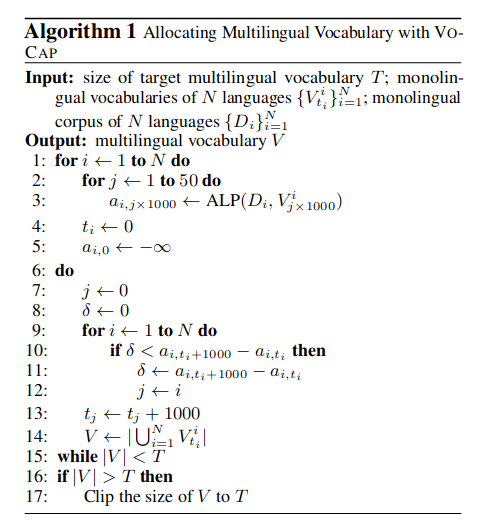
\includegraphics[width=0.8\textwidth]{img/temp/vocap_algo.png}
    \caption{\textsc{VoCap} algorithm pseudocode \cite{zheng_allocating_2021}. Figure taken from \cite{zheng_allocating_2021}.}
    \label{alg:vocab_allocation}
\end{figure}

With the \textsc{VoCap} algorithm \Citeauthor{zheng_allocating_2021} then create new tokenizers with vocabulary sizes 250\,000 and 500\,000 on a multilingual corpus with 86 languages. They compare the performance of the \textsc{VoCap} tokenizers with tokenizers trained directly on the multilingual corpus. The multilingual corpus is again subsampled before the standard tokenizer training following \citet{devlin_bert_2019,lample_cross-lingual_2019} with an exponential smoothing factor of $0.7$.

The standard and \textsc{VoCap} tokenizers are compared using the ALP metric. The authors show that the \textsc{VoCap} tokenizers improve the ALP metric for the 500\,000 vocabulary size over the baseline across all languages. The improvement is more prominent for low-resource and mid-resource languages compared to the high-resource languages. At the same time the difference between the standard tokenizers with vocabulary sizes 250\,000 and 500\,000 is not significant. The results are shown in \autoref{fig:alp_improvement}.

\begin{figure}
    \centering
    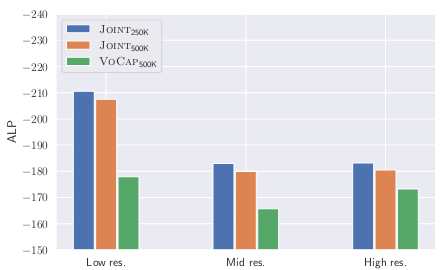
\includegraphics[width=0.8\textwidth]{img/temp/alp_improvement.png}
    \caption{ALP improvement of \textsc{VoCap} tokenizers over the standard tokenizers with vocabulary sizes 250\,000 and 500\,000. Figure taken from \cite{zheng_allocating_2021}.}
    \label{fig:alp_improvement}
\end{figure}

To validate these results, the authors then pretrain masked language models using the standard and \textsc{VoCap} tokenizers and conduct experiments on tasks from the XTREME benchmark \cite{hu_xtreme_nodate}. The comparison is done on natural language inference, paraphrase identification, part of speech tagging, named entity recognition and question answering. The averaged results over all tasks suggest that the \textsc{VoCap} tokenizers outperform the standard tokenizers by 0.4 percentage points for the 250\,000 vocabulary size and 1.7 percentage points for the increased 500\,000 vocabulary size. When investigating further the results for XNLI and NER, the authors show that the improvements are gained on the low-resource and mid-resource languages. This is consistent with the ALP improvement results.

% With the \textsc{VoCap} algorithm \Citeauthor{zheng_allocating_2021} then create new tokenizers with sizes 250k and 500k and show that for larger dictionaries (500k vocabulary size) their method outperforms the standard method of training a joint vocabulary on the union of the corpora. 


\subsection{Combination of methods for scaling the vocabulary size}

In the paper \Citetitle{liang_xlm-v_2023}, \citeauthor{liang_xlm-v_2023} propose a method for combining the two methods described above. 

\subsection{Other approaches}

- extending the vocabulary with new tokens
- multiview tokenization
- etc, go through my notes